\chapter{UML}

I diagrammi UML permettono di descrivere graficamente l'applicazione sotto vari punti di vista, garantendo la comprensione del funzionamento del software, delle esigenze che esso soddisfa e delle relazioni che intercorrono fra i suoi componenti.

Esistono diverse tipologie di diagrammi UML, quelle riportate nel presente documento sono:
\begin{itemize}
    \item diagramma dei casi d'uso
    \item diagramma delle attività
    \item diagramma degli stati
    \item diagramma delle classi
    \item diagramma di sequenza
\end{itemize}

Per ciascuno di essi verrà offerta una breve panoramica che includerà:
\begin{itemize}
    \item significato del diagramma 
    \item contesto in cui viene utilizzato
    \item funzionalità specifica dell'applicazione che viene descritta
    \item eventuali precisazioni/omissioni all'interno del diagramma e motivazione delle stesse
\end{itemize}

\newpage

\section{Use case diagram}

Lo use case diagram permette di identificare gli attori che interagiscono col sistema e le attività che essi possono svolgere. Lo scopo è descrivere le principali funzionalità del software.
Nel caso in esame:
\begin{itemize}
\item gli attori sono l'utente e l'applicazione stessa
\item i casi d'uso sono 
\begin{itemize}
\item gestione delle ricette e loro importazione/esportazione
\item gestione della lista della spesa
\item gestione della dispensa
\end{itemize}
\item ogni caso d'uso prevede la gestione degli errori che possono verificarsi, nonché l'esecuzione di alcune sub-routine necessarie per il corretto funzionamento dell'applicazione
\end{itemize}


\begin{figure}[H]
    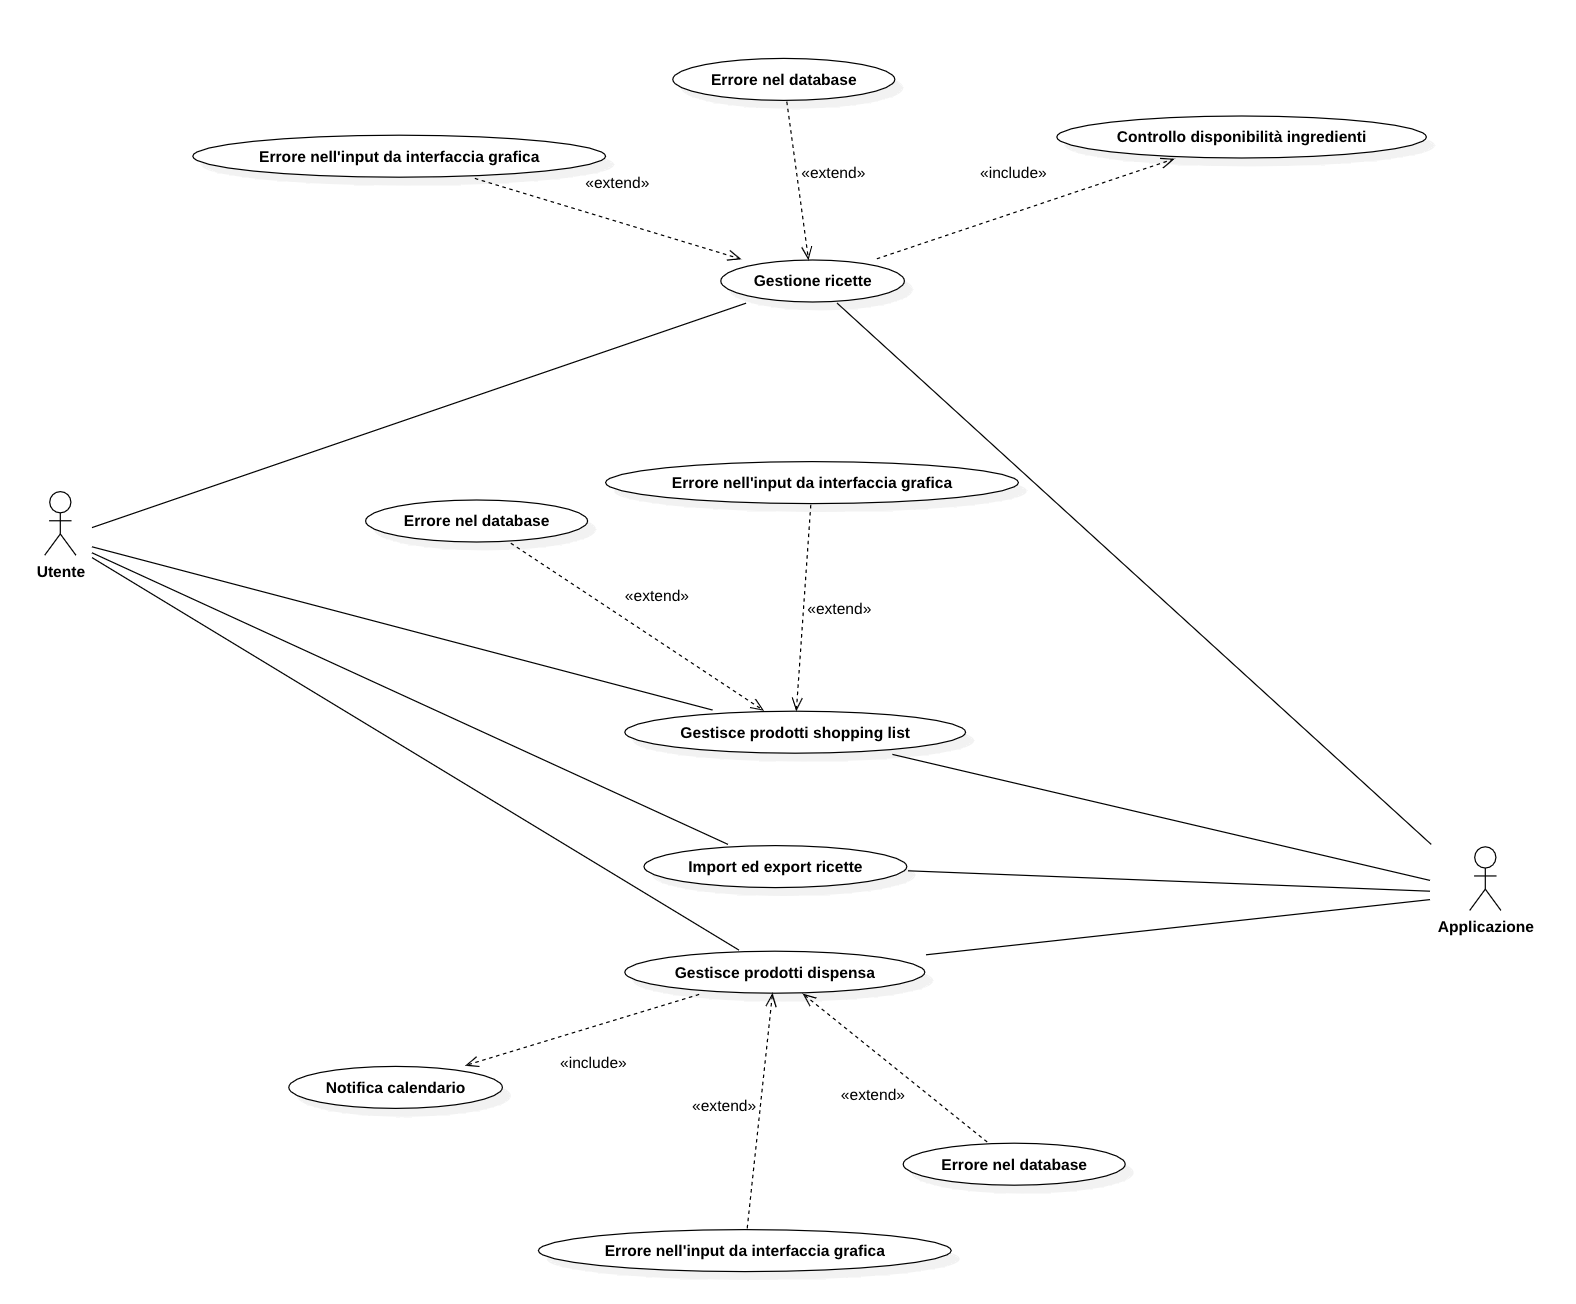
\includegraphics[width=\linewidth]{images/use-case.png}
    \caption{Diagramma dei casi d'uso.}
    \label{fig:usecase}
\end{figure}

\newpage

\section{Activity diagram}

L'activity diagram consente di specificare come il sistema realizzerà le funzionalità mostrate nello use case. Lo scopo è connettere tra loro azioni di alto livello per rappresentare un processo che viene svolto nel sistema. Per una migliore comprensione del funzionamento, nei diagrammi seguenti si è scelto di non modellare i casi di errore del database e dell'interfaccia grafica. 

\subsection{Activity diagram della dispensa}

In questo diagramma viene mostrato il processo relativo all'interazione fra l'utente e l'applicazione per la gestione della dispensa.
In particolare, le azioni dell'utente sul prodotto:
\begin{itemize} 
    \item sono propagate sia in memoria che sul database per garantire la consistenza dei dati
    \item hanno un impatto anche sulla generazione, modifica ed eliminazione delle notifiche sul calendario, per garantire che gli avvisi sulla scadenza dei prodotti siano coerenti con i dati dei prodotti stessi 
\end{itemize}

\begin{figure}[H]
    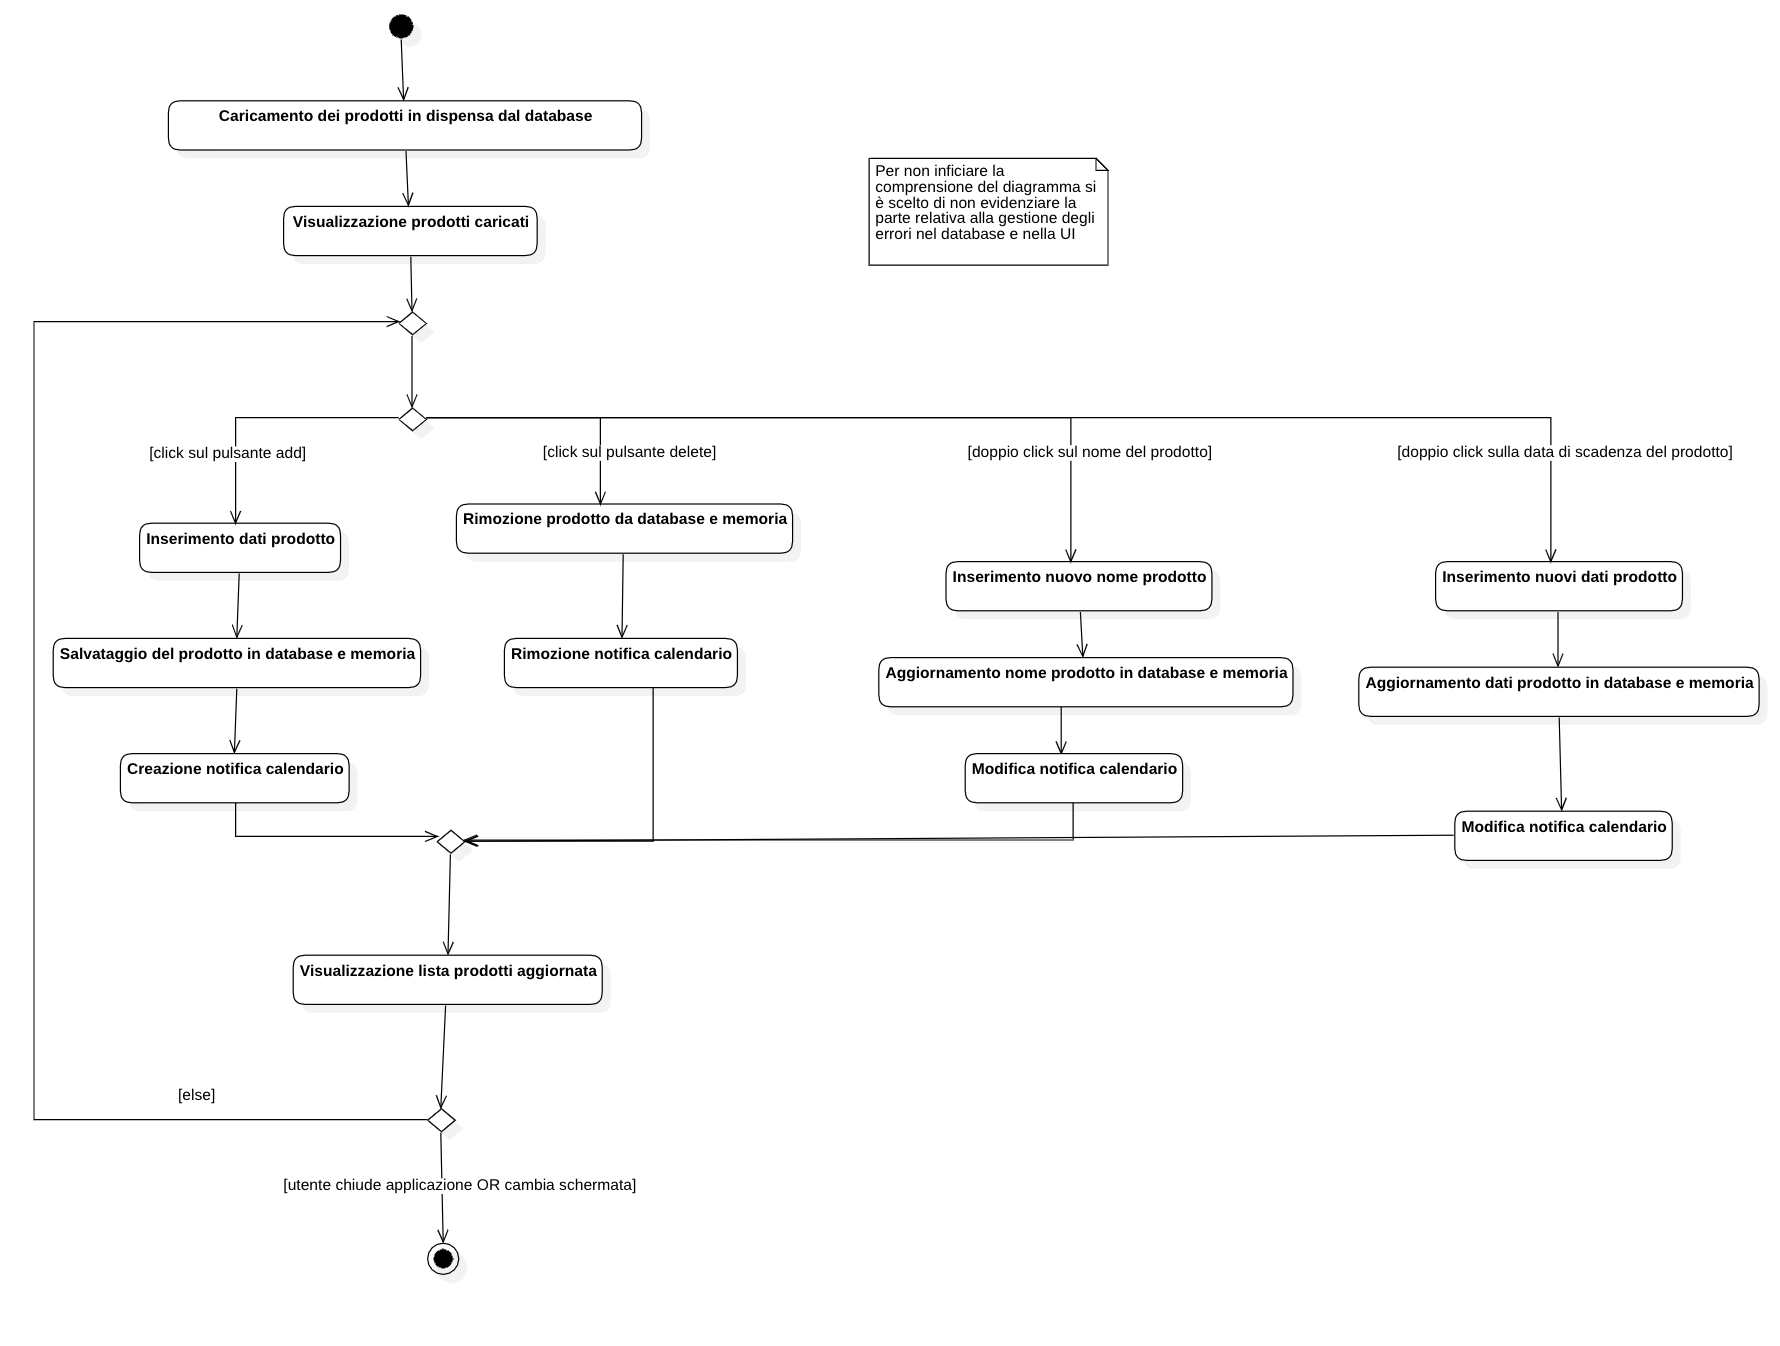
\includegraphics[width=\linewidth]{images/activity-pantry.png}
    \caption{Diagramma delle attività della dispensa.}
    \label{fig:actpantry}
\end{figure}

\newpage

\subsection{Activity diagram della lista della spesa}

In questo diagramma viene mostrato il processo relativo all'interazione fra l'utente e l'applicazione per la gestione della lista della spesa.
Si noti come:
\begin{itemize}
\item si faccia riferimento all'activity diagram precedente per evitare ripetizioni ed avere maggiore chiarezza in fase di modellazione e presentazione
\item rispetto al diagramma delle attività della dispensa, in questo caso si modella anche lo stato del prodotto, dal momento che esso può variare in base all'azione effettuata dall'utente
\item la struttura logica del diagramma sia molto simile a quella mostrata in precedenza, in quanto le azioni possibili sono quasi del tutto speculari
\end{itemize}

\begin{figure}[H]
    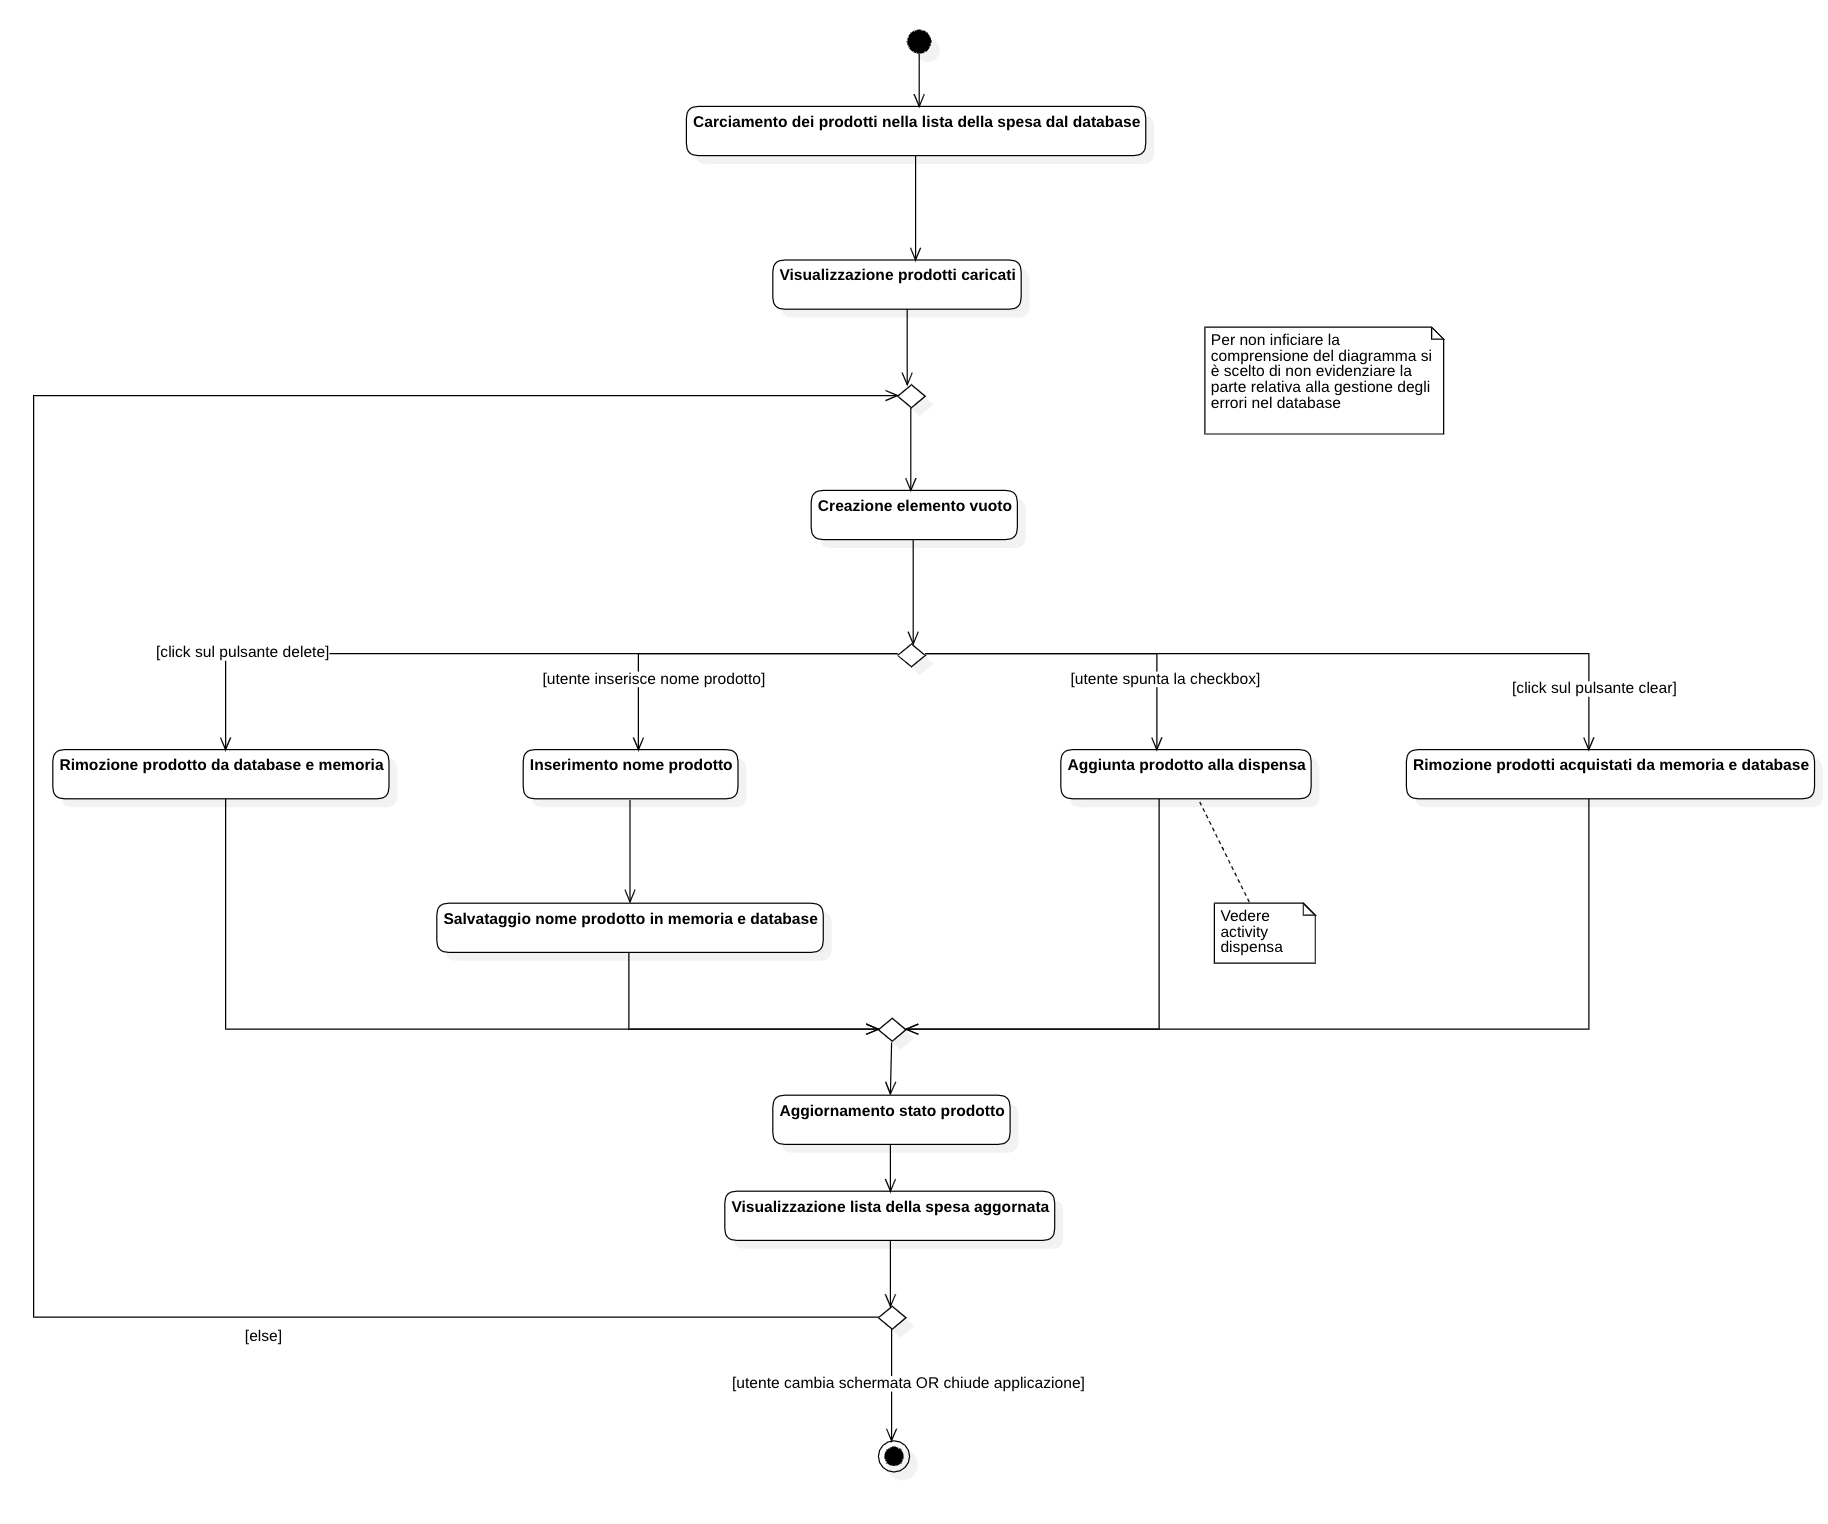
\includegraphics[width=\linewidth]{images/activity-shopping-list.png}
    \caption{Diagramma delle attività della lista della spesa.}
    \label{fig:actshoplist}
\end{figure}

\newpage

\subsection{Activity diagram delle ricette}

In questo diagramma viene mostrato il processo relativo all'interazione fra l'utente e l'applicazione per la gestione delle ricette, inclusa la possibilità di importare ed esportare ricette.
Elementi distintivi rispetto ai due casi precedenti sono:
\begin{itemize}
\item la distinzione fra le due possibili casistiche (nessuna ricetta disponibile oppure almeno una ricetta salvata nel database) in modo da poter mostrare all'utente il risultato più adatto alle sue necessità, come una ricetta vuota in cui inserire i dati nel caso non siano presenti ricette (caso che si verifica, per esempio, al primo avvio dell'applicazione)
\begin{itemize}
\item si noti come nel caso di ricetta presente nel database, venga eseguita anche la sub-routine relativa al controllo della disponibilità degli ingredienti in modo da fornire all'utente la consapevolezza circa l'effettiva realizzabilità del piatto
\end{itemize}
\item la già citata possibilità di importazione ed esportazione, utile per favorire la condivisione reciproca di ricette personali o di nicchia permettendone una rapida espansione 
\end{itemize}

\begin{figure}[H]
    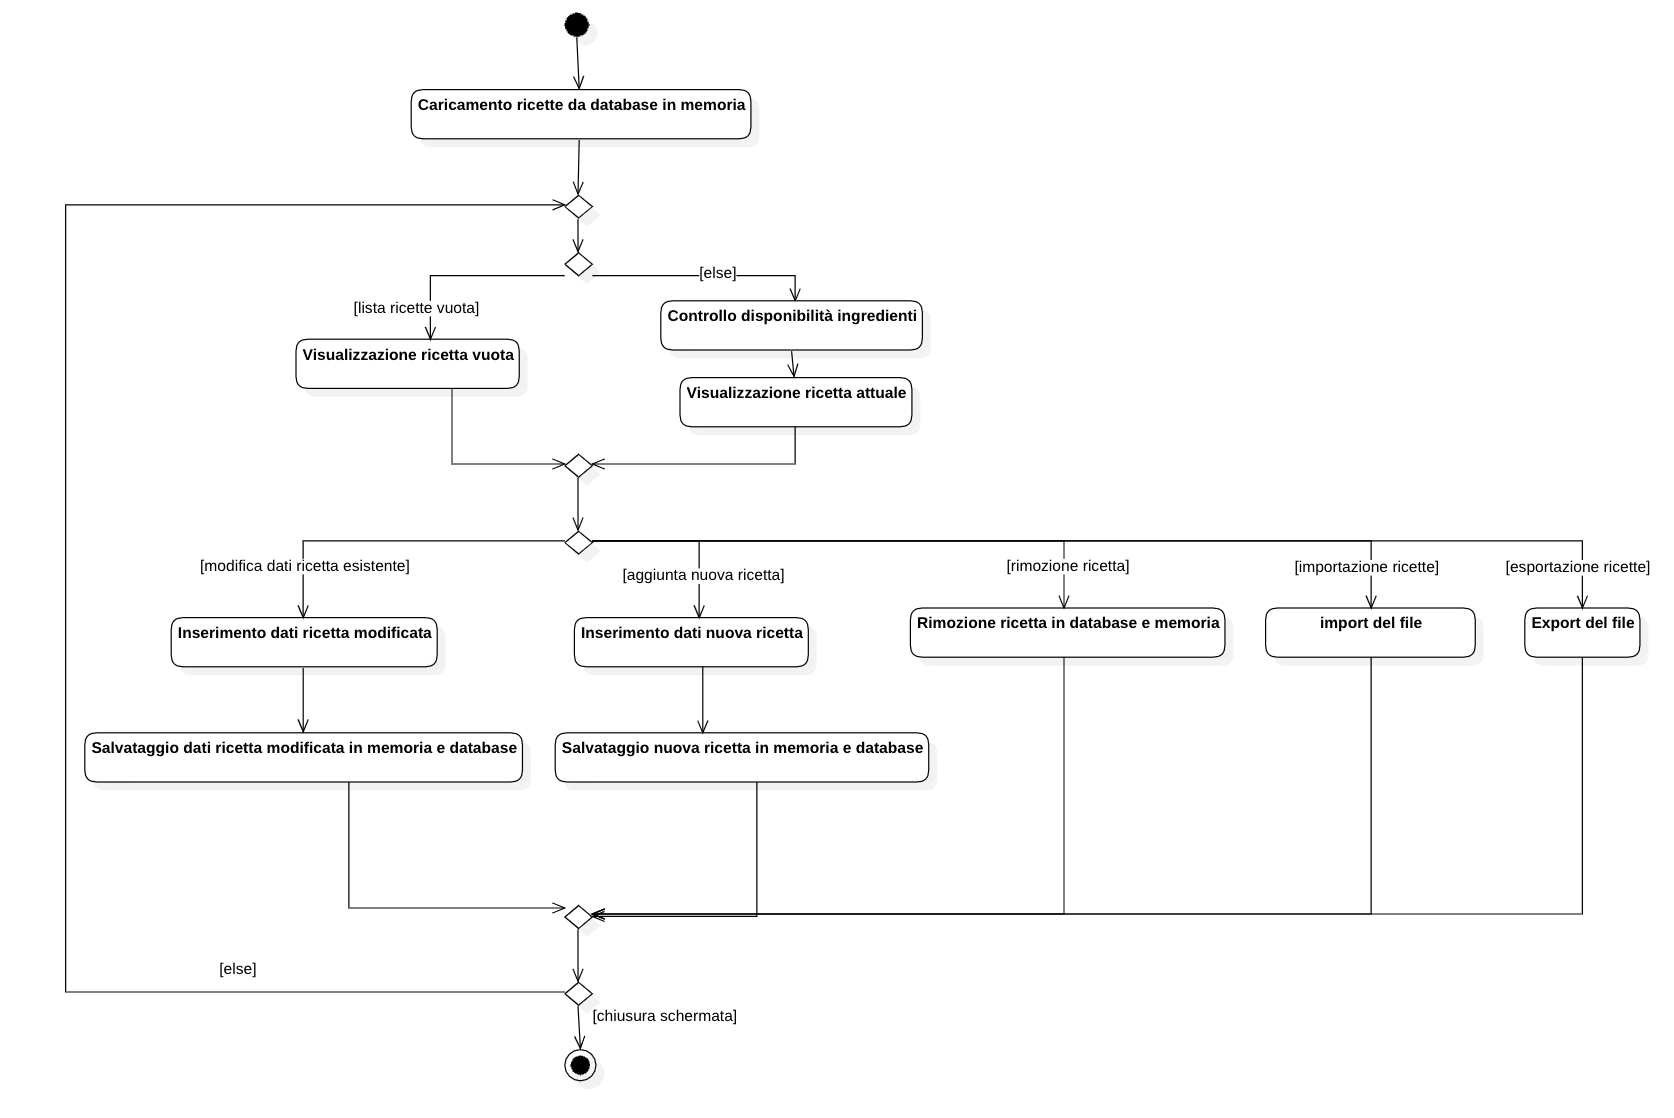
\includegraphics[width=\linewidth]{images/activity-recipe.png}
    \caption{Diagramma delle attività delle ricette.}
    \label{fig:actrecipe}
\end{figure}

\newpage

\section{State diagram}

Lo state diagram permette di modellare gli stati in cui si trova un oggetto e gli eventi che causano le transizioni fra gli stati. 

\subsection{State diagram della ricetta}

In questo diagramma vengono mostrati gli stati in cui si può trovare una ricetta in base alla presenza, e alla disponibilità, degli ingredienti.

\begin{figure}[H]
    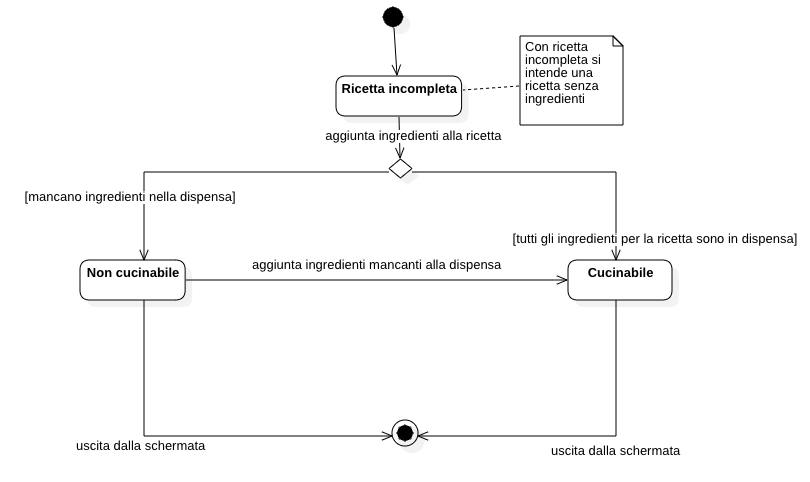
\includegraphics[width=\linewidth]{images/state-recipe.png}
    \caption{Diagramma degli stati della ricetta.}
    \label{fig:staterecipe}
\end{figure}

\newpage

\subsection{State diagram della lista della spesa}

In questo diagramma vengono mostrati gli stati in cui si può trovare un prodotto presente nella lista della spesa.

\begin{figure}[H]
    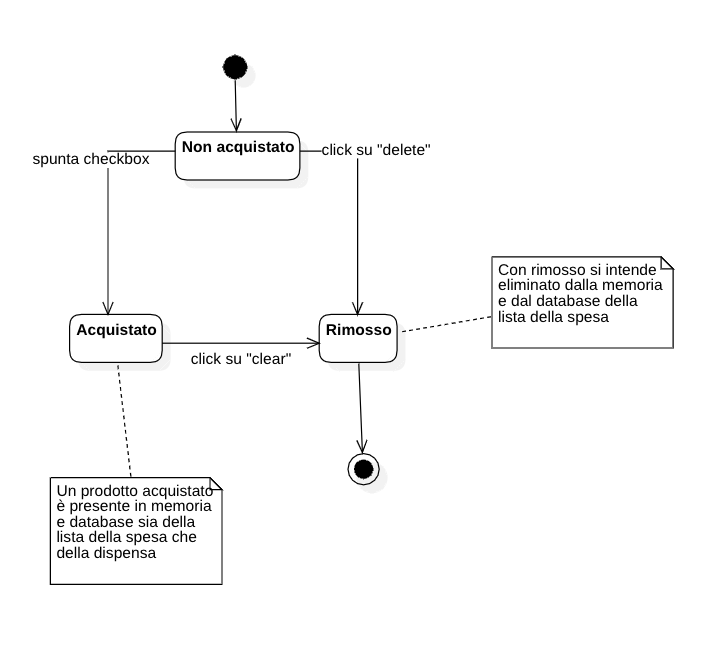
\includegraphics[width=\linewidth]{images/state-shopping-list.png}
    \caption{Diagramma degli stati della lista della spesa.}
    \label{fig:stateshoplist}
\end{figure}

\newpage

\section{Class diagram}

Il class diagram permette di descrivere i tipi di oggetti presenti nel sistema e le relazioni statiche che intercorrono tra di essi. Esso descrive inoltre gli attributi e i metodi di ogni classe, oltre ai vincoli che si applicano nel collegamento tra gli oggetti.

\begin{figure}[H]
    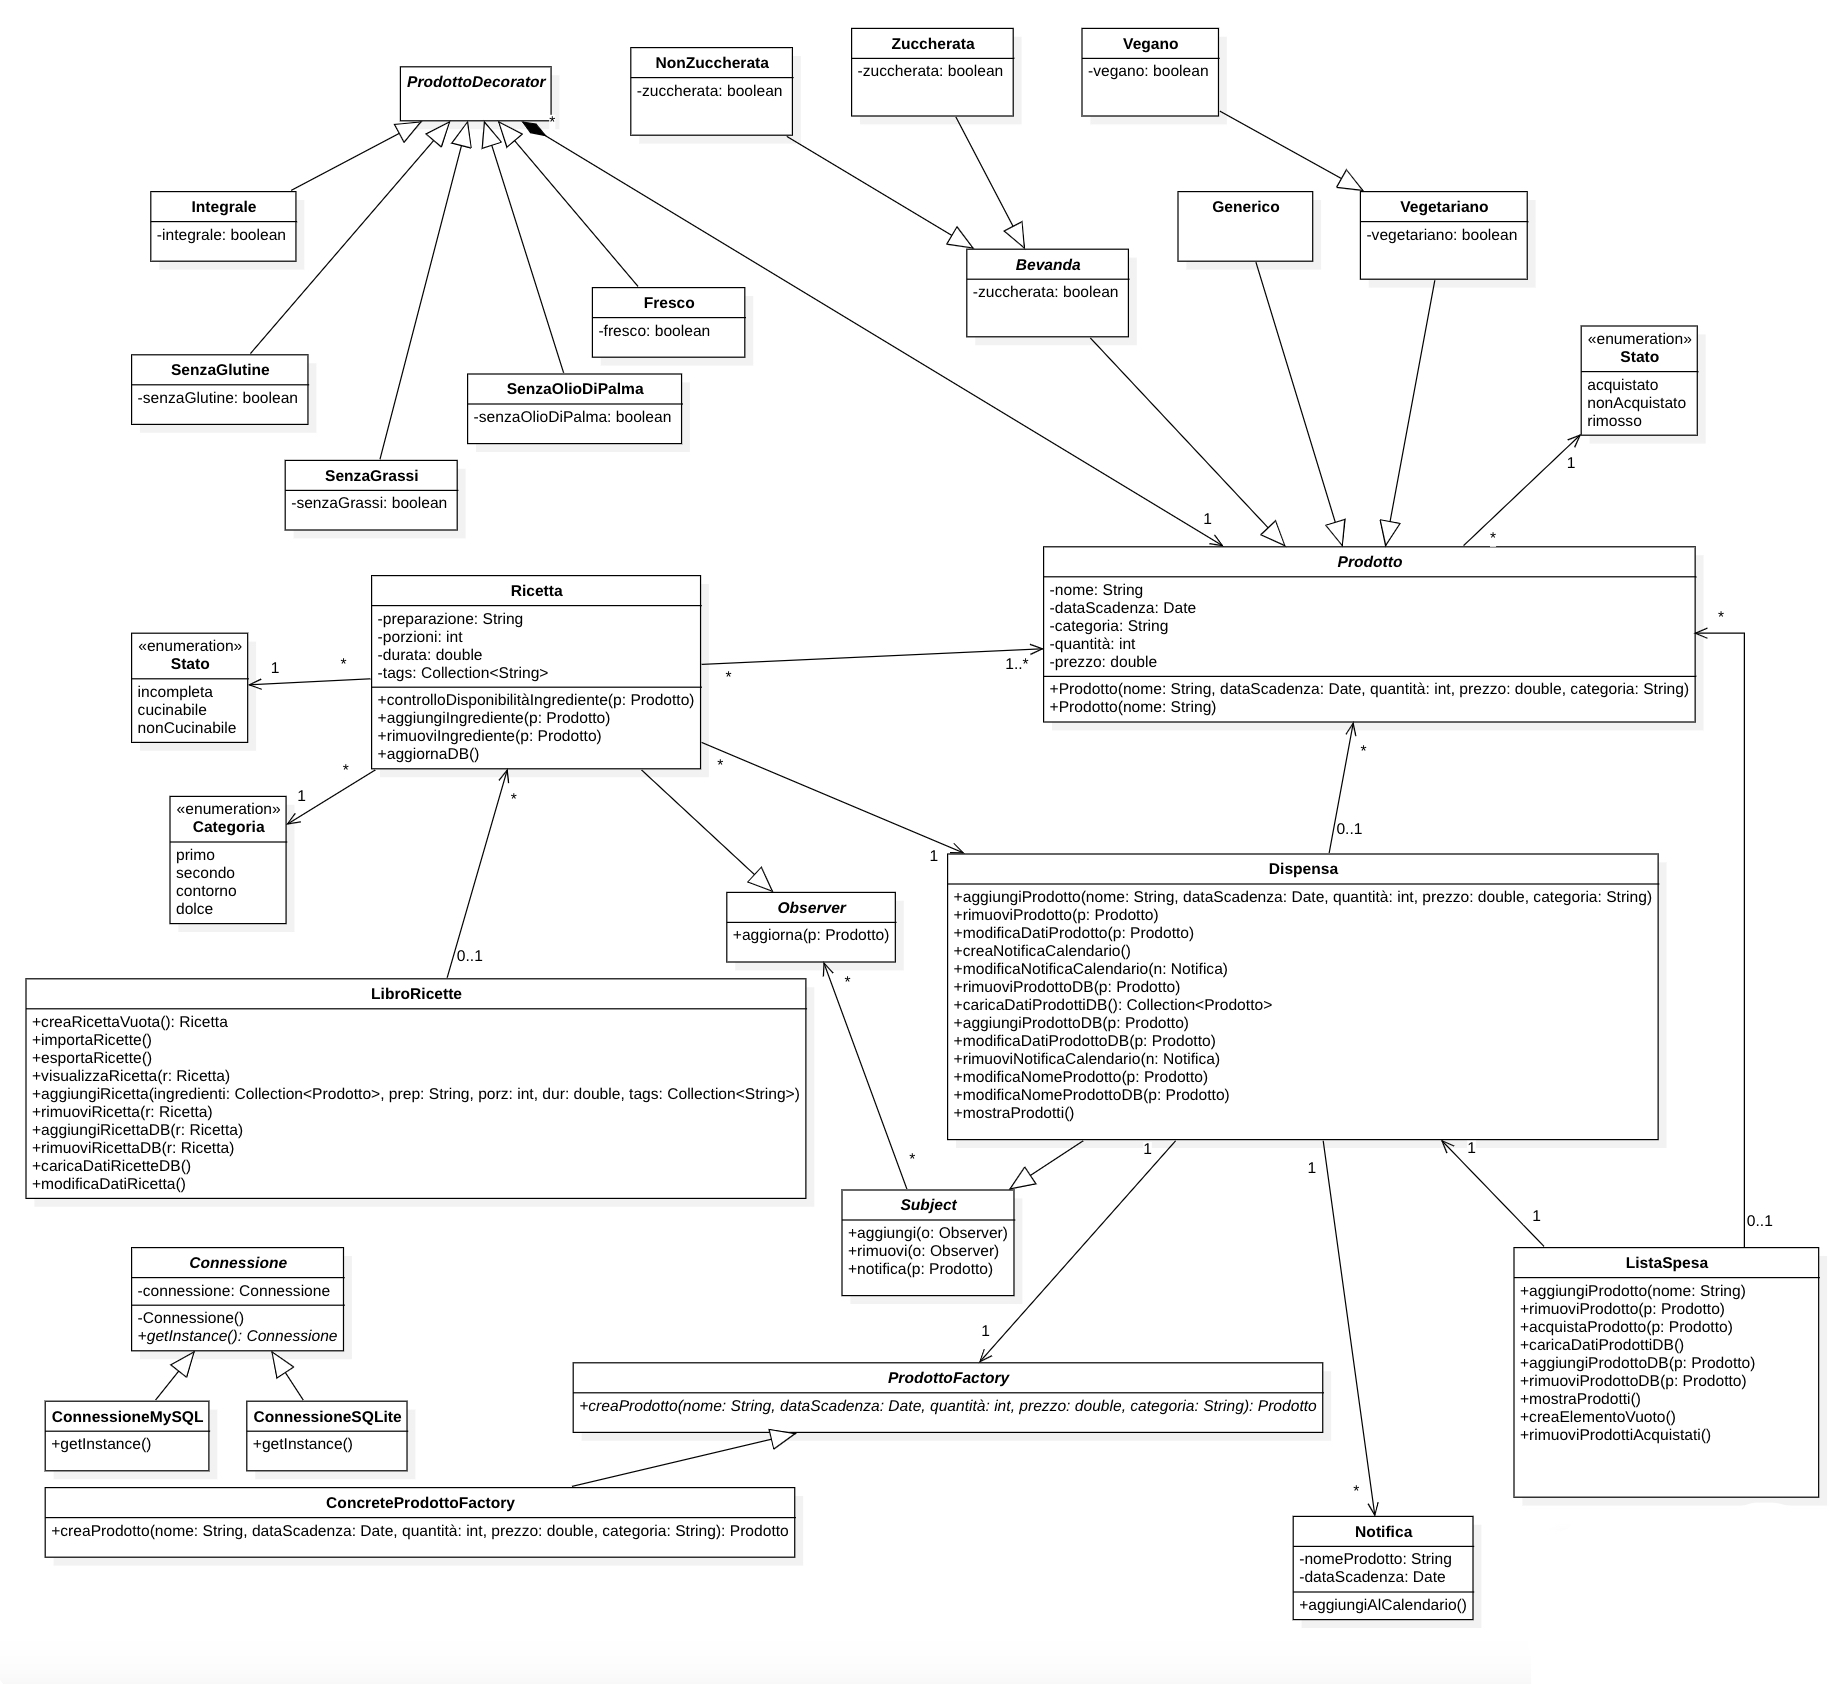
\includegraphics[width=\linewidth]{images/class.jpeg}
    \caption{Diagramma delle classi.}
    \label{fig:classdiagram}
\end{figure}

Per non complicare ulteriormente il diagramma si è scelto di non rappresentare la parte relativa all'interfaccia grafica. I design pattern applicati verranno spiegati nella sezione corrispondente.

\newpage

\section{Sequence diagram}

Il sequence diagram serve per descrivere singoli scenari dell'applicazioni. Lo scopo è mostrare come il sistema svolge le proprie funzioni. Per una migliore comprensione del funzionamento, nei diagrammi seguenti si è scelto di non modellare i casi di errore del database e dell'interfaccia grafica. 

Gli elementi principali di un sequence diagram, usati in tutti gli esempi successivi, comprendono:
\begin{itemize}
\item lifeline: rappresenta l'esistenza di un'entità in un dato istante della sequenza (utile quando un'entità è creata o eliminata durante una sequenza)
\item entità: attore/parte che interagisce con altri attori/parti; sono dotate di un nome ed eventualmente di una classe
\item messaggi: segnali che un partecipante (un'entità) invia ad un altro partecipante oppure provenienti da agenti esterni; possono essere specificati parametri, tipo del valore di ritorno
\item frammenti: operatori usati per modellare varie strutture di controllo, permettono di rappresentare molteplici flussi di esecuzione in maniera compatta e precisa
\item Esempi di frammenti utilizzati nei diagrammi seguenti
\begin{itemize}
    \item alt: rappresenta un \textit{if} con più condizioni (o \textit{guardie})
    \item opt: rappresenta un \textit{if} con una sola condizione
    \item loop: usato per modellare i cicli
\end{itemize}
\item Esempi di altri frammenti, usati per modellare l'ordine di esecuzione (seq, strict, par, critical) o l'occorrenza dei messaggi (ignore, consider, assert, neg)
\begin{itemize}
\item break: simboleggia la conclusione anticipata di un ciclo rispetto alla sua canonica esecuzione, spesso in seguito alla rilevazione di un'eccezione
\item seq: rappresenta l'ordinamento di default (ordinamento debole)
\item strict: rappresenta un ordinamento forte
\item par: permette di separare l'ordine degli operandi rendendoli indipendenti l'uno dall'altro (e potenzialmente eseguibili contemporaneamente)
\item critical: definisce un'area atomica nell'interazione, garantendo che essa non venga interrotta da eventi inaspettati
\item ignore: indica che il messaggio ricevuto è irrilevante
\item consider: indica che il messaggio ricevuto è di particolare importanza per l'interazione che si sta analizzando
\item assert: usato per definire situazioni che devono avvenire
\item neg: permette di modellare un'interazione invalida, come ad esempio i messaggi di errore
\end{itemize}
\end{itemize}

\subsection{Sequence diagram della dispensa}

\begin{figure}[H]
    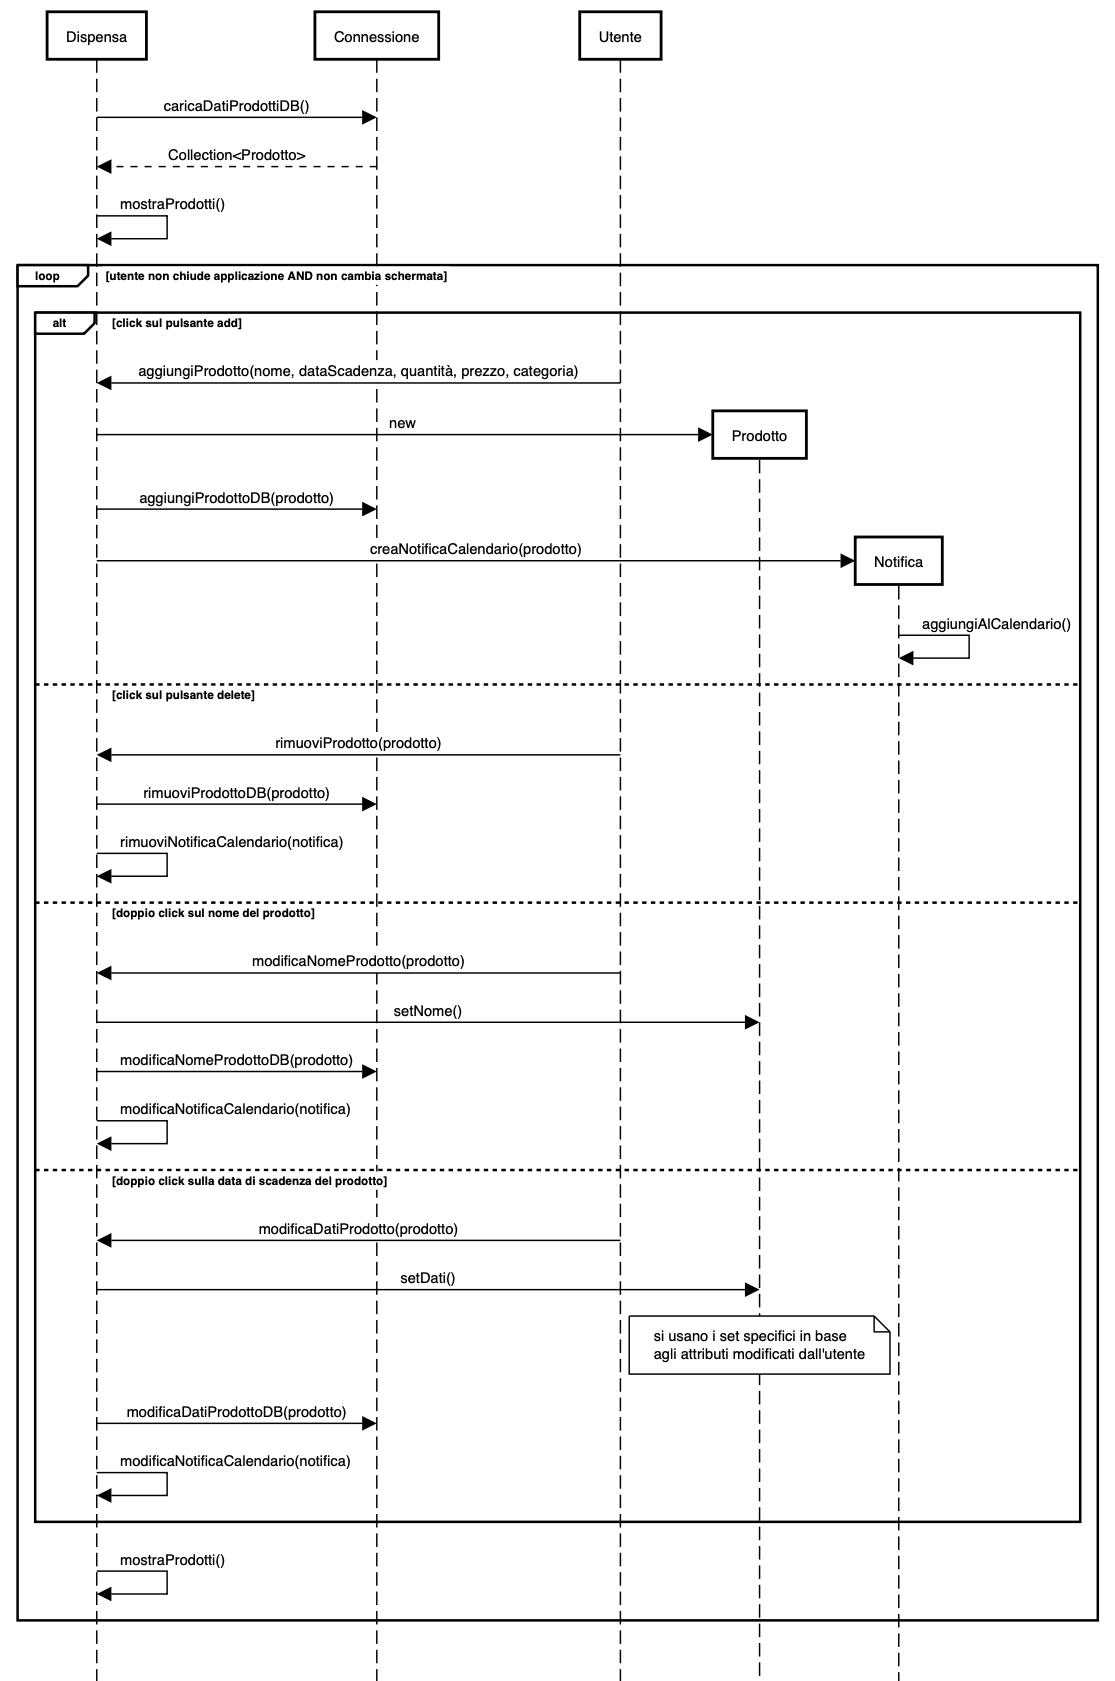
\includegraphics[width=\linewidth]{images/sequence-pantry.png}
    \caption{Diagramma di sequenza della dispensa}
    \label{fig:seqpantry}
\end{figure}

\subsection{Sequence diagram della lista della spesa}

\begin{figure}[H]
    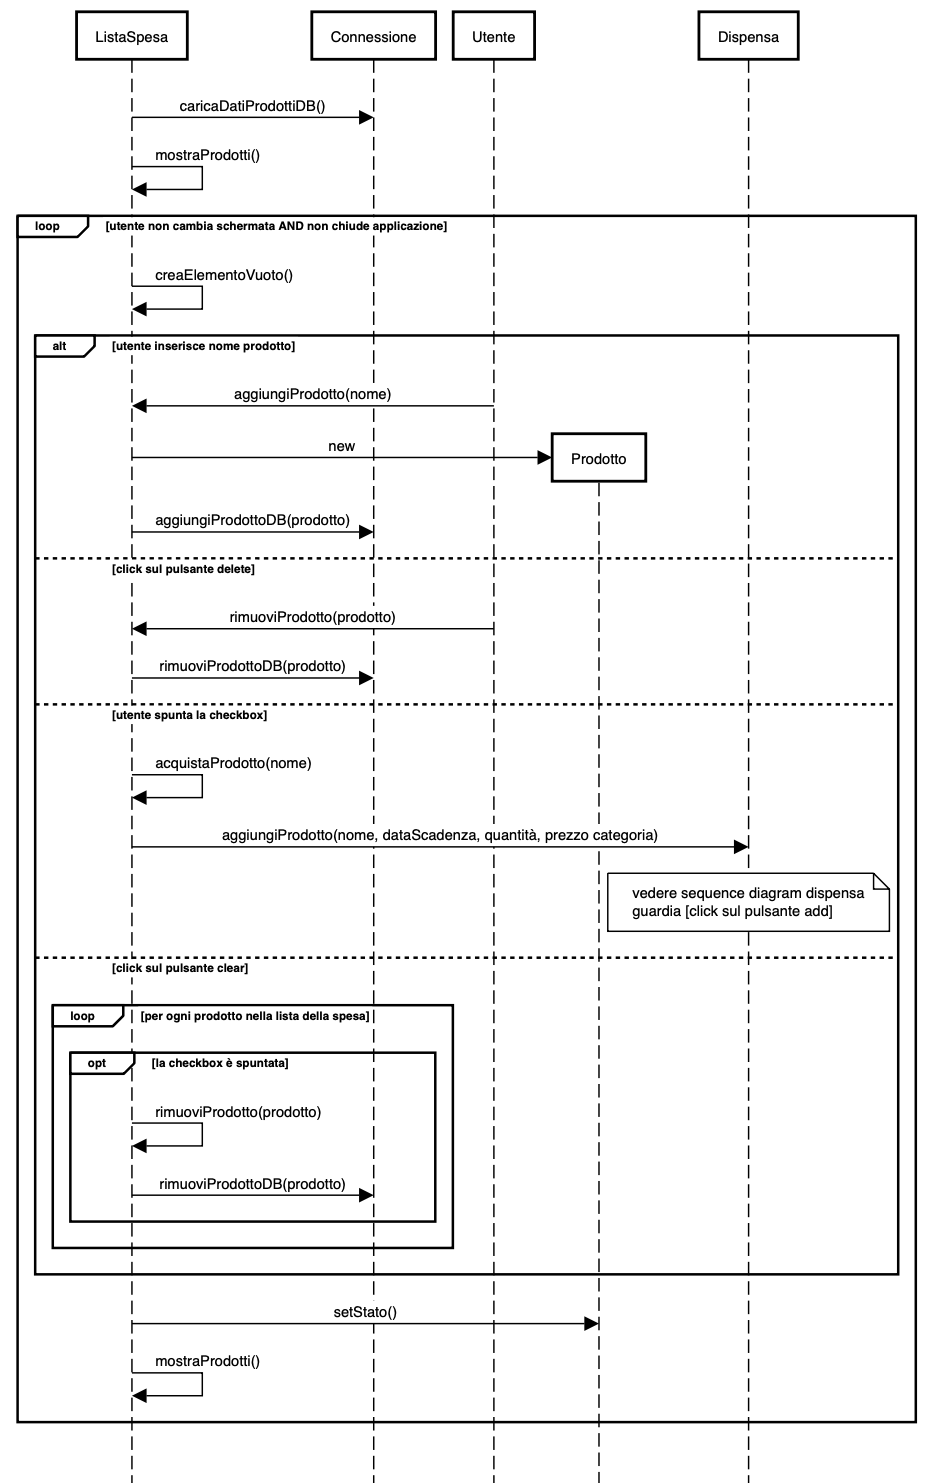
\includegraphics[width=\linewidth]{images/sequence-shopping-list.png}
    \caption{Diagramma di sequenza della lista della spesa}
    \label{fig:seqshoplist}
\end{figure}

\subsection{Sequence diagram delle ricette}

\begin{figure}[H]
    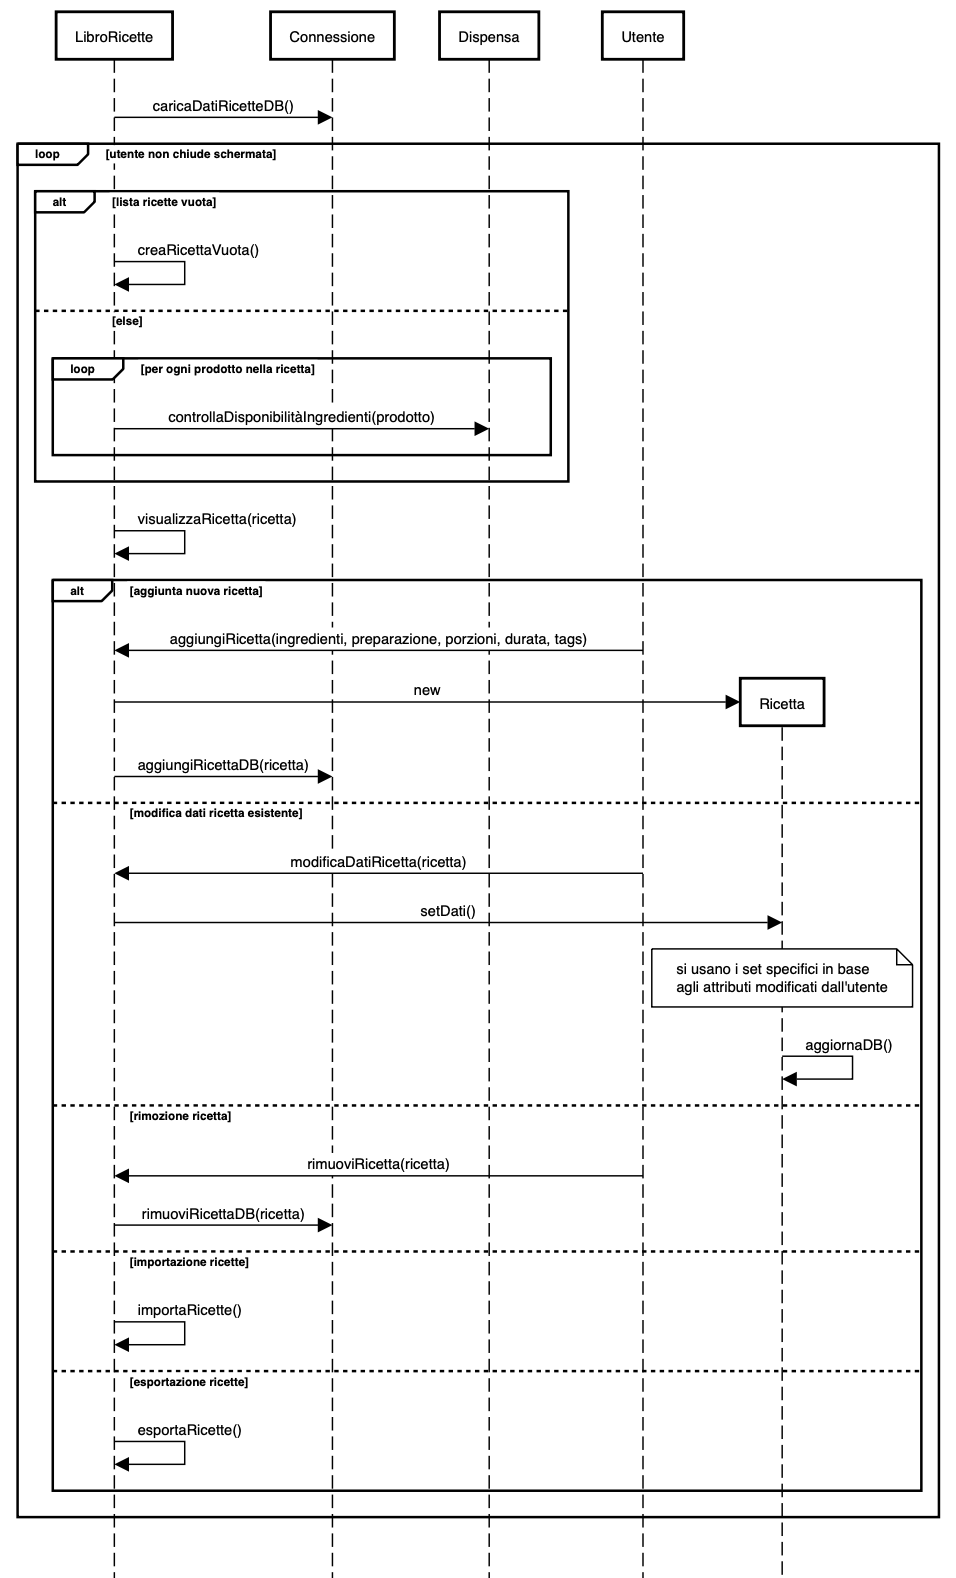
\includegraphics[width=\linewidth]{images/sequence-recipe.png}
    \caption{Diagramma di sequenza delle ricette}
    \label{fig:seqrecipe}
\end{figure}

Si noti che, per evitare sovrapposizioni nel diagramma che ne avrebbero resa più difficile la comprensione, il metodo \inlinecode{Java}{creaRicettaVuota()} (che si limita a mostrare dei campi di testo vuoti all'utente tramite l'interfaccia grafica) non crea un oggetto di tipo Ricetta (come invece avviene nel caso del metodo \\ \inlinecode{Java}{aggiungiRicetta(ingredienti, preparazione, porzioni, durata, tags)} in cui la ricetta creata presenta valori non nulli nei propri attributi).

